\section{Compiler} \label{section:compiler}

The first section of this paper describe the fluxionnal execution model, a framework to run web application in a distributed environment.
This section explains a method we developed to transform a subset of classic web application to be compliant with the execution model previously described.
This transformation unveils two problems.
A distributed system is defined in the first section by the parallel execution of its parts, and the independence of this parts from common memory.
While a classic web application is not composed of many independent parts, and relies on a central memory.
The problems are, firstly to parallelize the execution of a mono-thread application into many parts, and secondly to distribute the central memory among these independent parts.
\TODO{does it need a definition of the classic web application ? if so, should be in the introduction, not here}
We describe a compiler as a solution to this problems, hence capable to turn a classic web application into a scaling distributed system. \TODO{scaling is a bold claim, need some background}

The parallelization of a mono threaded program is a trending problem since the multiplication of the number of cores available on a machine.\TODO{references}
Asynchronism is different than parallelism, but in certain cases, one allow the other.
Promises\cite{Liskov1988} and Futures[??] are abstractions from an imperative, synchronous programing style, to an asynchronous execution model.
They transform synchronous, long waiting operations - like RPC or I/O - into asynchronous operations.
In a synchronous execution, the requested operation block the main thread until computation completes.
While in an asynchronous execution, the requested operation run along the main thread until the value is needed, releasing the main thread from waiting the operation to complete.
This asynchronism make the two execution paths independent, thus they can run in parallel until they are not independent enough - when one needs results from another.
We call rupture points, points where the execution flow forks in two independent and parallel paths.
These points mark out the limits between independent parts.

\TODO{next paragraph is a draft, needs rewrite}
Javascript is a functional and dynamically typed language initially introduced to handle user interactions within Web pages.
While Javascript isn't natively event-based, the DOM used in Web pages is.
The latter uses an event-loop to handle events happening on the Web page, and then triggers associated functions the developer provides.
\TODO{libevent, nginx : papers please ?}
\TODO{référence to interruptions}
More recently, \textit{Node.js} used the same event-loop based structure, to propose a non-blocking, event-based Javascript execution environment, specifically adapted for real-time I/O intensive applications like Web services.
Because of this event-loop based architecture, the I/O API \textit{Node.js} provides is non-blocking and asynchronous.
% The invocation of any function from this API returns immediately not to block the execution with time consuming I/O operations.
The developer provide an handler function as argument for this asynchronous function to invoke when the operation completes.
This handler function is commonly named a callback.%, \textit{Node.js} uses the convention to place the callback as the last parameter.
The \textit{Node.js} event-loop receives and gathers every I/O event, waiting its turn in the loop to invoke the associated callback.
% Listing \ref{lst:callback} illustrates the call of the asynchronous function \texttt{asyncFn} with the callback \texttt{callbackFn}.
% In most imperative languages the execution is synchronous by default, while special libraries handle parallelism, some using asynchronism like Promises and Futures cited above.
% However, 
\textit{Node.js} imposes natively both synchronous and asynchronous paradigms.
The asynchronous functions provided by \textit{Node.js} split the execution along two execution paths.
We defined rupture points in \textit{Node.js} as an asynchronous function call using a callback mechanism.
The two distinct execution paths are the synchronous instructions following the asynchronous function call, and the callback.
A rupture point marks out two independent parts of a web application.
One of the compiler step, the mapper, spot the rupture points, and split the application along them.

\TODO {References of solutions to split memory into distributed parts ?}
Parallelism is not sufficient for an application to be distributed, because of the central memory.
Promises and Futures don't transform a central memory into a distributed memory.
\textit{Node.js} provide a central memory, while the execution model expect it to be distributed into the application parts.
The compiler needs to split the shared memory into the application parts for the application to be compliant with the execution model previously described.

In Javascript, scopes are nested and only defined by functions.
Each function create a new scope containing variables local to itself.
This scope is chained to the scope of the parent function, so that the child function can access variables in the scope of the parent function, up to the global scope.
Callbacks defined inside a scope can access the same scope as the calling function, allowing them to share variables.
This feature is named closure.

Rupture points are always situated along scopes limits.
A scope is never shared between two application parts.
However, a child scopes separated in another application parts than its parent can't access the scopes it expects.
If the two scopes don't share the same memory, variables from the parent are unavailable for the child.
Another compiler step, the linker, understand and resolve dependencies conflicts between the distributed functions scopes.

In the next subsections, we describe the compilation steps.
The compiler uses program from the community, they are described in the first subsection along with the trivial compilation step.
Then, we describe two important compilation steps corresponding to the two previously described problems.
The \textit{mapper} breaks a program into many independent parts and the \textit{linker} resolves inconsistencies in the shattered memory scopes.

\subsection{Common tools : parser and code generation}

The first compilation step is to parse the source code taken as input.
The last compilation step is to output Javascript code either as a Javascript source code to run on the fluxionnal execution model, or as code in another high-level langage describing the fluxions and their content.
Parsing code and generating code back are common tasks.
There exist community projects to fulfill these tasks, like \textit{Esprima} and \textit{Acorn}, two Javascript parser.
For this compiler we use a serie of tool written by Ariya Hidayat and Yusuke Suzuki for the projects \textit{Esprima} and \textit{Esmangle}.
These tools follow the specification for an intermediate representation of the Javascript source code from the Mozilla Javascript Parser API : the Abstract Syntax Tree (AST)\footnote{\raggedright https://developer.mozilla.org/en-US/docs/Mozilla/Projects/SpiderMonkey/Parser\_API}.
This structured representation breaks the source into a tree of nodes, each representing a construct from the source, like an operation or an identifier.
It can be traversed and allow easy modification of its structure, without the risk of errors involved by direct source manipulation.

An example node in the AST is :

\begin{code}[Javascript, caption={Example of an AST node},label={lst:astnode}]
CallExpression {
    type: "CallExpression";
    callee: <Expression>;
    arguments: [ <Expression> ];
}
\end{code}

The compiler uses \textit{Esprima} to parse the source and generate the AST.
It is the first compilation step.
Thes AST can be traversed and explore with the use of \textit{Estraverse}.
\textit{Escope} detects function scopes and variables declaration using the previously generated AST, and output an object to represent the organisation of these scopes inside the source code.
One of the last compilation step is to produce a Javascript executable which uses the fluxionnal execution model.
To generate this Javascript code, the compiler use Escodegen, to transform back the AST into Javascript source code.

\subsection{Mapper : breaking the program}

The mapper detects rupture points, breaks the application into parts along them, and map every function scope to its corresponding application part.
Rupture points are indicated by calls of asynchronous function of higher order.

We distinguish specials rupture points indicated by asynchronous function handling series of external requests.
Unlike basic rupture points indicating an asynchronous continuity in the execution flow, the reception of an external request indicate the start of a virtualy new execution flow.
We distinguish these two types of rupture points to simplify later the dynamic analysis of system load.
Each new incoming request represent an additional load for the system, and is the main unpredictable factor.
While the incoming request load is taken into account, the load of every application part following in the continuity of the execution flow can be infered before run-time. 
The system load is only dependent at run time of the input in the system, everything else can be infered before run-time.
We explain this point in details in the next section of this paper.

These two types of rupture points corresond to different asynchronous functions in the \textit{Node.js} I/O API : the functions handling only one I/O event, or a bounded serie of I/O events, and the functions handling an unbounded serie of I/O events.

\subsubsection{One-time event} \label{sss:post}

Basic rupture points are indicated by asynchronous functions providing immediate I/O operation.
Callbacks of these functions are invoked only once, and continue the execution after the completion of the I/O operation.
Because of their asynchronism, these function calls mark the frontier between the current fluxion and the next one, inside a chain of fluxion.
The compiler replaces the asynchronous function call by a call to a placeholder function.
% This placeholder function uses the function \texttt{post(<msg>)} provided by the fluxionnal execution model described section \ref{section:model}.
% The placeholder function is detailed later, section \ref{ss:Scope}.

\subsubsection{Series of events} \label{sss:start}

Special rupture points are indicated by asynchronous functions providing a callback for a series of future event.
The handler of a network socket is called once for each incoming request.
The callbacks of these functions indicate the input of a data stream in the program, and the beginning of a fluxions chain.
As the callbacks mark the frontier between the current fluxion and the beginning fluxions chain, the compiler replaces the callback by a placeholder function starting the chain.
% This placeholder function uses the function \texttt{start(<msg)} provided by the fluxionnal execution model described section \ref{section:model}.
% The placeholder function is detailed later, section \ref{ss:Scope}.

The compiler uses a dictionnary of asynchronous functions to detect rupture points during the static analysis.
The compiler build this dictionnary when finding in the source, modules providing asynchronous function.
Such modules are \textit{Express} and \textit{fs}.
To find possible rupture points, the compiler tests the callee expression against this dictionnary for each callExpression node in the AST.

The compiler detects one rupture point for the following hello world web application. 

\begin{code}[Javascript, caption={Hello World},label={lst:hello}]
var app = require('express');
app.get('/', function(req, res) {
  res.send("Hello World :)");
});
\end{code}

% TODO insert the graph for this program

There is in this program only two scopes, the global scope, and the scope of the anonymous function.
These two scopes don't share any variable.

\subsection{Linker : resolving dependencies} \label{ss:linker}

In real world application, unlike in the previous example, the previously split applicaiton parts share variables, like the following example.
In this example web application, the two fluxions share a common variable : \texttt{rep}.

\begin{code}[Javascript, caption={Hello World with a shared variable},label={lst:sharedhello}]
var app = require('express'),
    rep = "Hello World :)";
app.get('/', function(req, res) {
  res.send(rep);
});
\end{code}

According to Brewer's theorem, formalized by Seth Gilbert and Nancy Lynch \cite{Gilbert2002}, a web application can only have two among the three options, Consistency, Availability, Partition tolerance.
As Coda Hale explained in one of his blog post\footnote{http://codahale.com/you-cant-sacrifice-partition-tolerance/}, network and node failures are unavoidable, a distributed system can't avoid to have failure.
Mike Stonebraker explain in another blog post\footnote{http://voltdb.com/blog/voltdb-products/clarifications-cap-theorem-and-data-related-errors/} that the trends is to make big data applications run on larger cluster of unreliable commodity machines.
Partition tolerance can't be avoided, so the only possible trade off is between consistency and availability.
These two tradeoff are defined in the literature as ACID (Atomicity, Consistency, Isolation, Durability) for consistency over availability, and BASE (Basically Available, Soft state, Eventual consistency) for availability over consistency.

If this trends is verified, transactional systems trading off availability for consistency, will become slower and slower.
It is hard to assure the atomicity of a transaction on a large cluster of machines, because it implies to block it [bullshit alert].
Choosing to sacrifice consistency might improve performance, without durable inconsistency in the datas.
It let design a lot more flexible solution, which have a better chance to cope with this kind of highly distributed architecture.


Dynamo system\footnote{http://s3.amazonaws.com/AllThingsDistributed/sosp/amazon-dynamo-sosp2007.pdf} already provides techniques to avoid complete chaos in a distributed system favoring availability.





While walking the AST, the compiler register every use of variables in a scope to determine what type of access is needed.
There is two type of access : read-only and modification.
To resolve the dependencies in a fluxion's signature, the compiler uses different techniques.

The variable is modified by one fluxion : Scope
The variable is modified by at least two fluxion : Sync
The variable is needed read-only by a downstream fluxion : signature
The variable is needed read-only by an upstream fluxion : ???? (lacking)


\subsubsection{Signature}

  The variables needed for read-only access by one of the scope of a fluxion and modified by another fluxion represent its signature.
  The signature of a fluxion is added in the message body between two fluxions.

  Every reference of this variable is replaced by a reference pointing in the signature part of the message.
  (basically reference -> msg.\_sign.reference)

  As a fluxion is only called on a message reception, the variable should never be lacking.
  If there is a problem in this situation, it is most likely a compilation error : the reference has not been replaced correctly, or the code is a corner case the compiler can't resolve yet.

\subsubsection{Scope}

  The scope of a fluxion holds the variables needed for modification, and never modified in another fluxion.
  Every reference of this variable is replaced by a reference pointing in the signature part of the message.
  (basically reference -> this.reference)
  If a variable in scope is read by another fluxion downstream, this variable is part of the signature of the downstream fluxion.

\subsubsection{Sync}

  If 

  If a variable is needed for modification by more than one fluxion, this variable needs to be synchronised between the fluxions.
  Here we want to apply some BASIC and Dynamo magic.



, the parent function sends the signature of the next fluxion in the same message together with the result of the asynchronous operation.
As the placeholder function call have the same scope than the asynchronous function call or callback it replaces, it is responsible for gathering the variables from the signature in a message along with the result of the operation and send it to the next fluxion.
The placeholder function call replacing \texttt{asyncFn} after compilation of listing \ref{lst:callback} is described in listing \ref{lst:placeholder}, line \ref{lst:placeholdercall}.

% \begin{code}[Javascript, caption={Example of a placeholder function call},label={lst:placeholder}]
% function MyFn() {
%   var a = 1,
%       b = 2,
%       c = 3;

%   // Placeholder for asyncFn-uid
%   flx.post(flx.m("asyncFn-uid", {a, b, c})); @\label{lst:placeholdercall}@
% }
% \end{code}







\subsection{Fluxionnal high level language printer}






\subsection{Fluxionnal execution model printer}



















% Stream line
As fluxions are chained one after another, a fluxion must provide every dependency for the next one, even if some of this dependencies miss from its own scope or signature.
These dependencies must be passed fluxion after fluxion from the producing fluxion, to the consuming fluxion.
So, the message stream linking one fluxion to another includes the signature of the next fluxion as well as dependencies targeting downstream fluxions.
The compiler has to resolve the content of these message streams beginning by the last fluxions and going upstream to the first ones.
Figure \ref{fig:streamline} illustrate this principle : since fluxion \textit{C} needs the variable \textit{z}, fluxion \textit{B} needs the variable \textit{z} as well to pass it along to fluxion \textit{C}.

\begin{figure}[h!]
  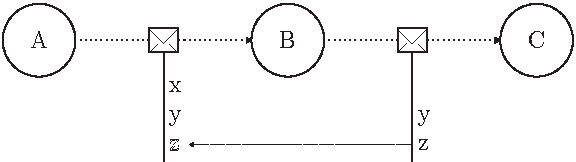
\includegraphics[width=\linewidth]{ressources/streamline.pdf}
  \caption{Fluxion C needs the variable z, so does fluxion B}
  \label{fig:streamline}
\end{figure}

\subsection{Limitations} \label{ss:Limitations}

% For example, functions from the \texttt{Array} prototype ask functions as parameters for a behavior to call on each iteration over the array.
% Listing \ref{lst:array} presents an example of this structure.
% This iteration is synchronous, so the function passed as an argument, \circled{1}, and the code following the function call, \circled{2}, are somehow dependent.
Leaving an asynchronous function call as is doesn't introduce bugs, however breaking a synchronous function by replacing its callback leads to bugs.
To avoid introducing new bugs, it is important for the compiler to be able to distinguish between these synchronous and asynchronous functions.

% \begin{code}[Javascript, caption={Example of a synchronous function using a callback},label={lst:array}]
%   my_modified_array = my_array.map(function(element) {
%     // Modifying element @\Comment{\circled{1}}@
%   })
%   // Following code @\Comment{\circled{2}}@
% \end{code}

% Problem with dynamically typed functions

% Functions are of higher order in Javascript, so arrays can contain functions, as well as a variables.
Javascript is dynamically typed, if the index to access an array can't be resolved statically, then so do the type of the result.
Some callbacks can't be resolved statically.
For example, in listing \ref{lst:unresolved}, the function \texttt{myAsyncFn} is asynchronous and ask for a callback as parameter.
The compiler would break the program along its call, however \texttt{event.type} is unresolvable statically, the compiler is unable to include the callback in the next fluxion.
This structure might already be encapsulated inside a fluxion, and the callback might need variables from the scope of an upstream fluxion, but as the callback is unresolved, it is impossible for the compiler to track them, and add these dependencies in the signature of the current fluxion.
Even if the compiler leaves this structure as is, it introduce dependency bugs as the compiler is unable to resolve dependencies and generate accurate signatures.
The compiler is currently unable to compile a program containing structures involving dynamic resolution like in listing \ref{lst:unresolved}.

\begin{code}[Javascript, caption={Example of an unresolvable callback},label={lst:unresolved}]
myHandlers = [];
// ... definition of myHandlers
onEvent(function(event) {
  myAsyncFn(myHandlers[event.type])
})
\end{code}


\subsection{Futur Works}

Even synchronous, the use of a callback by the \texttt{map} function indicate an independence between the callback and the main execution thread.
For future improvements, we focus on studying these independences to allow the compiler to spot and break into fluxions these patterns of synchronous function call using callbacks.

For future improvements, we focus on a solution to dynamically compile fluxions and resolve dependencies, allowing to compile programs containing dynamic structures described in the last paragraph.

% \subsection{Compilation example}

% As of today our work on the compiler is still incomplete, there is inconsistencies between the high-level language detailed in section \ref{section:model} and the compilation results.
% For documentation purposes, this section details the compiler current state of progress.

% Listing \ref{lst:compsource} is a simplified version of the example listing \ref{lst:classique} in section \ref{section:model}.
% We use this simplified version as a test for our compiler, as it is yet unable to handle dynamic resolution, like used with the object \texttt{count} line \ref{lst:classique_dynres} in listing \ref{lst:classique}.
% The result of this compilation is listing \ref{lst:comptarget}.
% In the compilation result, the fluxion \textit{id-1000} should hold a context containing the variable \texttt{count}, like the object \texttt{uid} in the context of fluxion \textit{logic}, listing \ref{lst:fluxionnal}.
% But our compiler is yet unable to correctly resolve dependencies and fluxion contexts, so this counter service is unable to increment visits.

% \begin{code}[Javascript, caption={Simplified version of the initial service},label={lst:compsource}]
% var app = require('express')();
% var count = 0;

% app.get("/:id", function id(req, res){
%   count = count + 1;
%   res.send(count);
% });

% app.listen(8080);
% \end{code}

% \begin{code}[Javascript, caption={Compilation result of code listing \ref{lst:compsource}},label={lst:comptarget}]
% // Main >> id
%   var flx = require('fluxion');
%   var app = require('express')();
%   var count = 0;
 
%   app.get("/:id"n function placeholder(req, res) {
%     flx.start(flx.message("id-1000", {
%       res: res,
%       count: count
%     }))
%   })
 
%   app.listen(8080);

% // id-1000
%   flx.register("id-1000", function id-1000(msg){
%     res.send(msg.count = msg.count + 1);
%   })
% \end{code}





